%%%%%%%%%%%%%%%%%%%%%%%%%%%%%%%%%%%%%%%%%%%%%%%%%%%%%%%%%%%%%%%%%%%
%%% Documento LaTeX 																						%%%
%%%%%%%%%%%%%%%%%%%%%%%%%%%%%%%%%%%%%%%%%%%%%%%%%%%%%%%%%%%%%%%%%%%
% Título:		Capítulo 3
% Autor:  	Ignacio Moreno Doblas
% Fecha:  	2014-02-01, actualizado 2019-11-11
% Versión:	0.5.0
%%%%%%%%%%%%%%%%%%%%%%%%%%%%%%%%%%%%%%%%%%%%%%%%%%%%%%%%%%%%%%%%%%%
% !TEX root = A0.MiTFG.tex

\section{Tercera iteración: Rendimiento}
    \subsection{Resumen}
        
        Con esta iteración se pretende añadir todo lo referente a las mediciones de rendimiento del algoritmo. Tratando de concluir el prototipo inicial. Esta iteración aún se centrará exclusivamente en la funcionalidad del proyecto dejando de lado todas las cuestiones referentes a diseño de interfaces y experiencia de usuario para iteraciones posteriores.
        
    \subsection{Requisitos}

        Los requisitos a realizar en esta iteración son el 1.3.3 y el 1.3.4 de la tabla inicial (Tabla \ref{tab:Requisitos}) junto al requisito 2.5 de la tabla completa (TODO: Referencia tabla final) añadido durante la iteración anterior. Para ello se divide el trabajo de la iteración en las siguientes tareas:

        \begin{enumerate}
            \item Aislamiento del procesado de señales en una tarea exclusiva.
            \item Extraer las medidas de rendimiento del sistema operativo.
            \item Mostrar dichas medidas en el panel de usuario de QT.
        \end{enumerate}
        
    \subsection{Desarrollo}
        
        El procesado de la señal se ha movido de la rutina encargada de manejar las comunicaciones, donde se alojaba inicialmente de forma provisional, a una tarea propia, desde la que resulta más sencillo calcular el tiempo de procesado y determinar los recursos que están siendo consumidos por la misma. Además independizar estas dos tareas también ayuda a descongestionar las comunicaciones entre el dispositivo y el panel de control. Sin embargo con la adición de las funciones necesarias para el funcionamiento de la tarea se carga de contenido el fichero que finalmente será editable por el usuario, por este motivo, se ha decidido crear un fichero dedicado exclusivamente a las funciones del usuario llamado UserEntry.c y su correspondiente fichero de encabezado UserEntry.h, facilitando así la implementación de los algoritmos a evaluar. 
        
        Con los cambios incurridos en esta tarea, el diagrama de flujo del ciclo de trabajo del dispositivo de pruebas queda conforme a la figura \ref{fig:tivaFlow}. Aunque se debe tener en cuenta que en realidad las diferentes tareas mostradas en el diagrama no se ejecutan de forma perfectamente secuencial. El diagrama es solo una representación gráfica del flujo de una iteración completa de la ejecución en un caso ideal. En la realidad es posible que lleguen comandos mientras se ejecuta el algoritmo de detección. Para gestionar estas interrupciones el sistema operativo usa las prioridades.
        
        \begin{figure}
                \centering
                        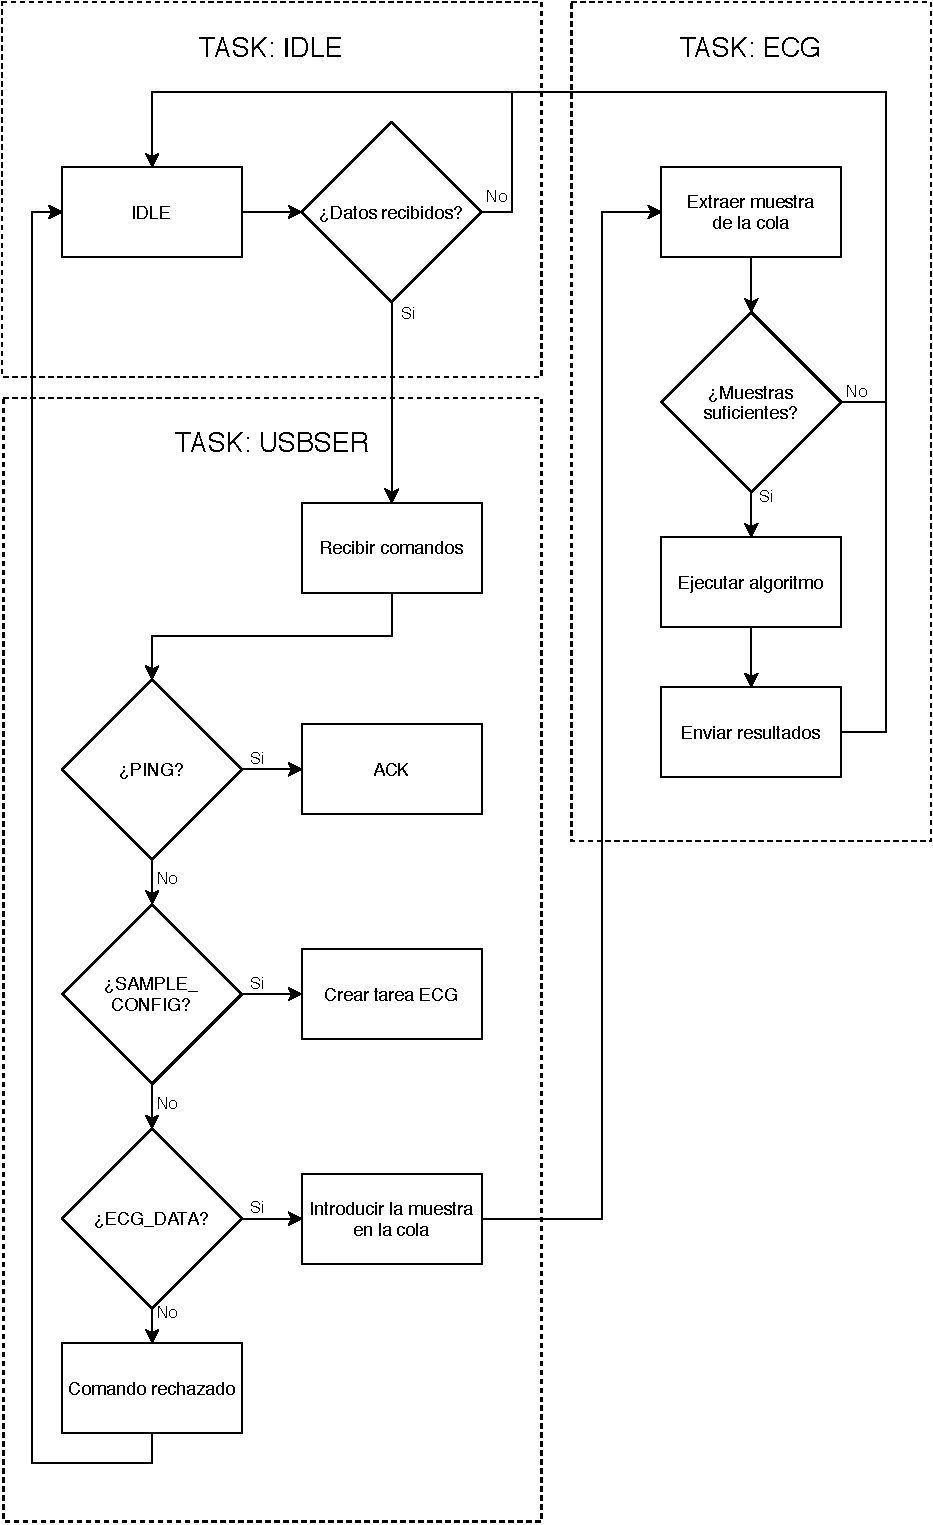
\includegraphics[width = 0.78 \linewidth]{figuras/TivaWorkFlow.pdf}
                \caption{Diagrama de flujo de las tareas en ejecución del dispositivo de pruebas.}
                \label{fig:tivaFlow}
        \end{figure}
        
        Para la realización de la segunda tarea se ha empleado un Timer de alta frecuencia del dispositivo para contar el número de ciclos de reloj empleados en llevar a cabo cada ciclo de ejecución del algoritmo. El Timer empleado es el Timer4 configurado en modo cuenta periódica de 32 bits ascendente. Para realizar la medida al comienzo de cada ciclo de procesado se le asigna el valor 0 y cuando el procesado concluye se consulta la cuenta del temporizador, siendo esta equivalente al numero de ciclos de reloj transcurridos en el proceso. Si este valor se divide entre la frecuencia del mismo se obtiene una medida del tiempo empleado. La implementación puede observarse en la figura \ref{fig:timer}.
        
        \begin{figure}[H]
                \centering
                        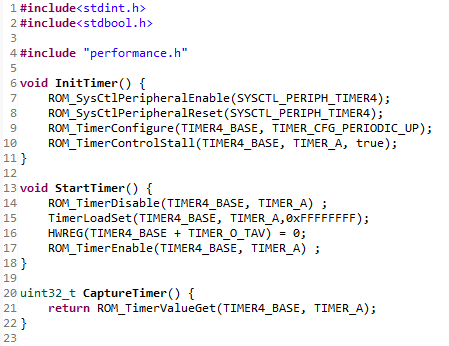
\includegraphics[width = 0.7 \linewidth]{figuras/Timer.PNG}
                \caption{Implementación del Timer de diagnóstico.}
                \label{fig:timer}
        \end{figure}
        
        Con un objetivo similar también se hace uso de la función ``vTaskGetInfo()'', perteneciente al sistema operativo, para extraer datos del estado de la CPU y el uso de memoria de la tarea de procesado. A diferencia del tiempo medido con el timer los datos de uso de CPU extraídos con esta función no son exactos pero si suficientes para dar una idea general de la carga de trabajo. Respecto a la memoria, se indica la cantidad de memoria libre de la que dispone la tarea, por lo que valores altos son ideales, si este número llegara a cero significaría que la tarea se ha desbordado. 
        
        Para mostrar las medidas de rendimiento al usuario en el panel primero era necesario enviarlas, y para ello se ha decidido emplear otro paquete diferente al de los resultados del algoritmo. De esta forma se evita sobrecargar un paquete que ya es de por sí bastante grande y además se consigue independencia previendo que en alguna iteración posterior se puedan añadir nuevos indicadores de rendimiento, que pueden incluso no depender de la ejecución del algoritmo.
        
        Respecto a la visualización de los datos, de momento solo se han añadido las salidas de texto correspondiente con la mínima explicación necesaria, posponiendo los detalles de interfaz de usuario para más adelante. Los valores son expuestos de manera visual y agrupada para su fácil comprensión, siguiendo el ejemplo de la figura \ref{fig:performance}.
        
        \begin{figure}[H]
                \centering
                        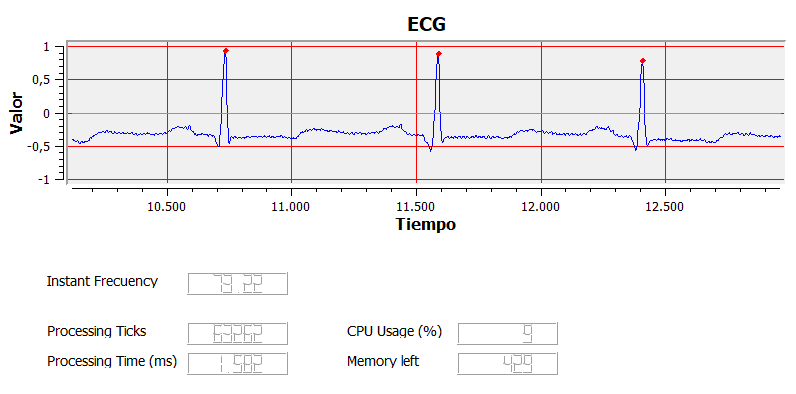
\includegraphics[width = 0.9 \linewidth]{figuras/Performance.PNG}
                \caption{Visualización de los datos de rendimiento.}
                \label{fig:performance}
        \end{figure}
        
    \subsection{Pruebas}
        
        De las tareas realizadas en esta iteración, la única que requiere de pruebas es la extracción de los datos de rendimiento de la CPU, concretamente el caso de la implementación del timer. Para ello se ha empleado la función ``SysCtlDelay()'' capaz de introducir un retardo fijo en la ejecución de una tarea. Midiendo el tiempo introducido por dicha función empleando el timer podemos obtener garantías de que la medida se está llevando a cabo correctamente. Como se puede ver en la figura \ref{fig:performanceTest} la medición obtenida es coherente con los datos introducidos.
        
        \begin{figure}[H]
                \centering
                        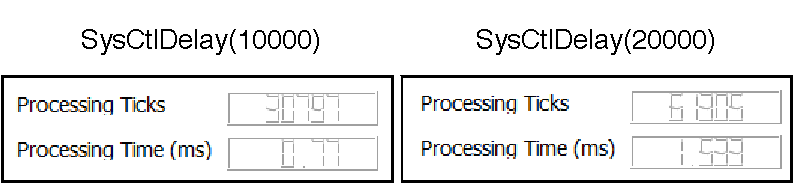
\includegraphics[width = 0.9 \linewidth]{figuras/PerformanceTest.pdf}
                \caption{Prueba medición tiempo de ejecución del algoritmo.}
                \label{fig:performanceTest}
        \end{figure}

    \subsection{Conclusiones}
    
        Después de invertir bastante tiempo en las funciones de diagnostico del sistema operativo en tiempo real para realizar las medidas de rendimiento estas han demostrado ser bastante imprecisas, especialmente aquellas dedicadas a medir las cargas de CPU. Pues todas se basan en un contador desde el momento en que se inició el sistema, por lo que si las tareas no se ejecutan a pleno rendimiento desde el comienzo los promedios van a estar muy desviados de la realidad, o por el contrario, van a tardar bastante tiempo en dar un resultado estable.